\chapter{External Comparisons, Competitive ETAS Benchmarks, Robustness, and Sequence Concentration}
\label{ch:external}
\section{Study overview}

The stronger benchmark defeats the target procedure in both external regions: fitted inverse-power ETAS (EP) exceeds Omori continuous (OC) on joint score in every primary California and Japan test window (while losing one episode in the separate five-episode causal-window backtest in Section~\ref{sec:s06-completed}). OC nevertheless improves California timing against fixed-scale Mittag-Leffler continuous (FC) by 0.119969 nats per target and location against the coarse Omori cell-lift (OL) by 2.140710, over 315 targets. These are different references, and the location gain primarily measures recovery of within-cell density. Japan retains that representation contrast but reverses the OC--FC timing direction in every window, so the registered combined transfer criterion is not demonstrated. California's positive timing contrast is strongly concentrated in one eligible sequence period. Conditional diagnostics also expose OC discrepancies. These inspected and revised archives support retrospective fitted-procedure comparisons, not pristine confirmation or a physical mechanism.

\section{Question, status and relation to the preceding work}

The question is how far the specific forecasting improvements reported in Chapter~\ref{ch:nz-spatial} travel when the region, comparator and diagnostic question change. There are four distinct questions: does a matched ablation retain its direction elsewhere; does the complete procedure beat serious alternatives; do its conditional probabilities resemble the recorded history; and where do the realised score differences occur? A positive answer to one does not answer the others.

Chapter~\ref{ch:nz-spatial} found a large location-score advantage for continuous offspring geography over a cell-lift representation in New Zealand, and a smaller timing advantage for Omori decay over fixed-scale Mittag-Leffler decay within the continuous representation. Its 612 historical targets are context for the programme, not an additional denominator for any table below. The present chapter consolidates subsequent completed studies. Chapter~\ref{ch:local-inhibition} separately reports the local-inhibition extension and its negative observed result. The original manuscript and Addenda I--III remain historical source authorities; the present chapter integrates the completed studies into this unified monograph.

The historical comparisons in this chapter are supported by retained fit, score and audit records. The current public reproduction bundle supplies the recovered catalogue inputs and original fitted states; the reproduction guide identifies each independently executed replay.

\section{Models, forecast object and score}

\subsection{Arm names and what each comparison changes}

The abbreviations are local procedure names, not claims of new model families. All excitation arms share the declared training-only magnitude recipe with productivity exponent r = 0.7 and score the magnitude mark once.

\begingroup\small\setlength{\tabcolsep}{2pt}\renewcommand{\arraystretch}{1.18}
\begin{longtable}{@{}>{\raggedright\arraybackslash}p{0.2280\textwidth}>{\raggedright\arraybackslash}p{0.2280\textwidth}>{\raggedright\arraybackslash}p{0.2280\textwidth}>{\raggedright\arraybackslash}p{0.2280\textwidth}@{}}
\toprule
{}Arm & Temporal law & Offspring geography & Role \\
\midrule\endfirsthead
\toprule
Arm & Temporal law & Offspring geography & Role \\
\midrule\endhead
\midrule\multicolumn{4}{r}{\emph{Continued on next page}}\\
\endfoot
\bottomrule\endlastfoot
{}FC & Fixed-scale Mittag-Leffler & Continuous OC geography & Primary timing reference \\
{}FL & Fixed-scale Mittag-Leffler & Cell-lift & Spatial/context reference \\
{}MC & Free common-scale Mittag-Leffler & Continuous OC geography & Temporal context \\
{}OC & Omori & Continuous OC geography & Frozen target procedure \\
{}OL & Omori & Cell-lift & Primary location reference \\
{}EP & Omori ETAS adaptation & Unweighted inverse-power radial law & Competitive reference \\
{}N0 & No offspring excitation & Smooth background & Refitted no-trigger reference \\
{}LI & Omori plus immigrant attenuation & Continuous OC geography & Inhibition extension in Chapter~\ref{ch:local-inhibition} \\
\end{longtable}\endgroup

The continuous OC offspring density multiplies a radial factor by a fixed training-derived reference density and normalizes over the finite domain separately for each parent. A cell-lift uses target-cell-centre weights and spreads each cell's offspring mass uniformly inside it; actual parent coordinates remain in the calculation. Thus OC-OL is a particular within-domain representation comparison. Both retain smooth immigrant geography. EP instead uses a separately fitted, pure inverse-power offspring kernel, normalized with respect to projected area without OC's reference-density multiplier. OC-EP compares whole procedures with different spatial laws; it is not an isolated temporal-kernel experiment.

The cell-lift and national-routing arms are coarse representation controls. Their losses establish the cost of those discretizations for the declared score, rather than competitive superiority over an equally resolved alternative. The separately fitted EP arm supplies the stronger spatial comparison. Keeping the testing population, forecast object and reference explicit follows the forecast-evaluation distinction emphasized in CSEP methodology \citep{Schorlemmer2007,Zechar2010}.

N0 fixes branching at zero and refits its own background time-rate parameters on training data. It is neither an OC fit with its trigger switched off afterwards nor a constant-Poisson numerical floor. LI attenuates only the immigrant component of OC; its full definition and exact zero-inhibition nesting are given in Chapter~\ref{ch:local-inhibition}.

\subsection{Sequential conditional forecasting}

At each origin, parameters and spatial nuisance choices use training data only and remain fixed during the test window. Every strictly earlier admissible observed event can enter the subsequent history, including earlier events in that test window. This scores a sequential conditional forecast. It does not supply the whole future catalogue at the origin, and it is not an issue-frozen nonhomogeneous Poisson forecast of the complete future path.

The finite domain, parent eligibility, exposure and projected-area measure are shared within each contrast. For an event intensity \(\lambda(t,z)\), its regional ground intensity \(R(t)\), full space-time exposure \(E\), and common magnitude-mark score \(M\), define

\begin{align}
P&=\sum_i\log\lambda(t_i,z_i),&Q&=\sum_i\log R(t_i),\\
E&=\int_{I}\int_D\lambda(t,z)\,\mathrm dz\,\mathrm dt,&C&=-E,\\
S_{\rm time}&=Q+C,&S_{\rm loc}&=P-Q,\\
S_{\rm joint}&=P+C+M=S_{\rm time}+S_{\rm loc}+M.
\end{align}

Higher is better. In a difference between procedures, the signed exposure contribution is minus the difference in E. Quiet periods therefore contribute even when they contain no targets. Common mark differences cancel; a positive location difference is not a statement about magnitude forecasting. Nats are natural-log score units, not percentage accuracy, correlations, causal effects or an estimated percentage of predictable earthquakes. Pooled nats per target divide the sum of window differences by the sum of target counts, never the unweighted average of window means.

This event-logsum and compensator construction is a logarithmic point-process score (the negative of an entropy-loss convention); its differences express log-score gain for the declared observation law \citep{DaleyVereJones2004}.

These symbols are the narrative convention throughout Chapters~\ref{ch:external}--\ref{ch:local-inhibition}. The source-field dictionary maps legacy labels without changing their values: LI's raw pooled key E denotes a point-logsum difference, while sequence timing\_\allowbreak{}compensator denotes a signed difference in nonnegative integrated exposure whose score contribution has the opposite sign. Neither raw name overrides the definitions above.

Primary timing means OC-FC timing; primary location means OC-OL conditional location. These rows use different references and cannot be added to manufacture a combined gain. A direct OC-FL joint contrast, where reported, is a separate comparison.

\section{California: successful matched transfer with uneven contributions}

\subsection{Population and chronological windows}

The repaired California source contains 1,272 canonical unique preferred SCEDC/SCSN records meeting reported M $\geq$ 4.0, latitude 32-37 degrees, longitude -121 to -114 degrees and depth -5 to 40 km. Of these, 106 records in 1981-1985 provide warmup parents. Scored training begins in 1986; expanding training prefixes contain 851, 930 and 1,097 targets. The three half-open UTC test windows contain 79, 167 and 69 targets. Their total is 315 unique held-out targets. Reappearance of this denominator in the benchmark, calibration, concentration and inhibition studies reflects reuse of those same targets, not new samples.

The schema repair retained an earlier stop and changed only acceptance of unused location-quality metadata as opaque printable tokens. All 45 cached official files were reused unchanged; no query, row removal, imputation or forecasting-engine change was needed. The 134 previously rejected occurrences were retained, and none was an M $\geq$ 4 model candidate. Independent reconstruction established equality of the previous model and diagnostic arrays. This establishes lossless handling within the verified snapshot, not universal source completeness or uninspected historical forecasting.

\subsection{Primary results}

\begingroup\footnotesize\setlength{\tabcolsep}{2pt}\renewcommand{\arraystretch}{1.18}
\begin{longtable}{@{}>{\raggedright\arraybackslash}p{0.1800\textwidth}>{\raggedright\arraybackslash}p{0.1800\textwidth}>{\raggedright\arraybackslash}p{0.1800\textwidth}>{\raggedright\arraybackslash}p{0.1800\textwidth}>{\raggedright\arraybackslash}p{0.1800\textwidth}@{}}
\toprule
{}Window (targets) & OC-FC timing nats & Timing nats/target & OC-OL location nats & Location nats/target \\
\midrule\endfirsthead
\toprule
Window (targets) & OC-FC timing nats & Timing nats/target & OC-OL location nats & Location nats/target \\
\midrule\endhead
\midrule\multicolumn{5}{r}{\emph{Continued on next page}}\\
\endfoot
\bottomrule\endlastfoot
{}2011-2016 (79) & +0.099084 & +0.001254 & +91.803255 & +1.162067 \\
{}2016-2021 (167) & +32.722878 & +0.195945 & +465.829993 & +2.789401 \\
{}2021-2026 (69) & +4.968377 & +0.072005 & +116.690274 & +1.691163 \\
{}Pooled (315) & +37.790339 & +0.119969 & +674.323522 & +2.140710 \\
\end{longtable}\endgroup

Both primary directions are positive in all three windows. Timing is nearly tied in the early window; the middle window supplies about 87\% of the total timing difference. The timing pair also has a negative conditional-location difference in the middle window. Positive primary directions therefore do not imply uniformly improved components or a constant effect size.

Of the +674.323522 conditional-location nats, +653.602228 come from within-cell density. This is consistent with the distinction between a continuous density and uniform within-cell offspring mass. It does not establish a similarly large gain in allocation among broad zones or cells, nor general accuracy of individual event locations. Training selected both background bandwidth and inherited offspring scale at 5 km, the lower grid endpoint in every California fold. This is a boundary of the declared grid, not an identified physical interaction distance or proof of coordinate accuracy.

Thus about 96.93\% of this location contrast comes from within-cell density. The analogous higher-threshold share is about 95.48\%. These large shares are consequences of the particular uniform-within-cell reference; they are not percentages of correctly predicted locations or evidence of a physical interaction distance.

For context, OC-MC gains +21.177884 joint nats (+0.067231 per target), FC-FL gains +671.244340 location nats (+2.130934), and the direct OC-FL comparison gains +747.800021 joint nats (+2.373968). Each wins all three windows. Their reference arms and score components differ; these results are not additive.

\begin{figure}[tbp]\centering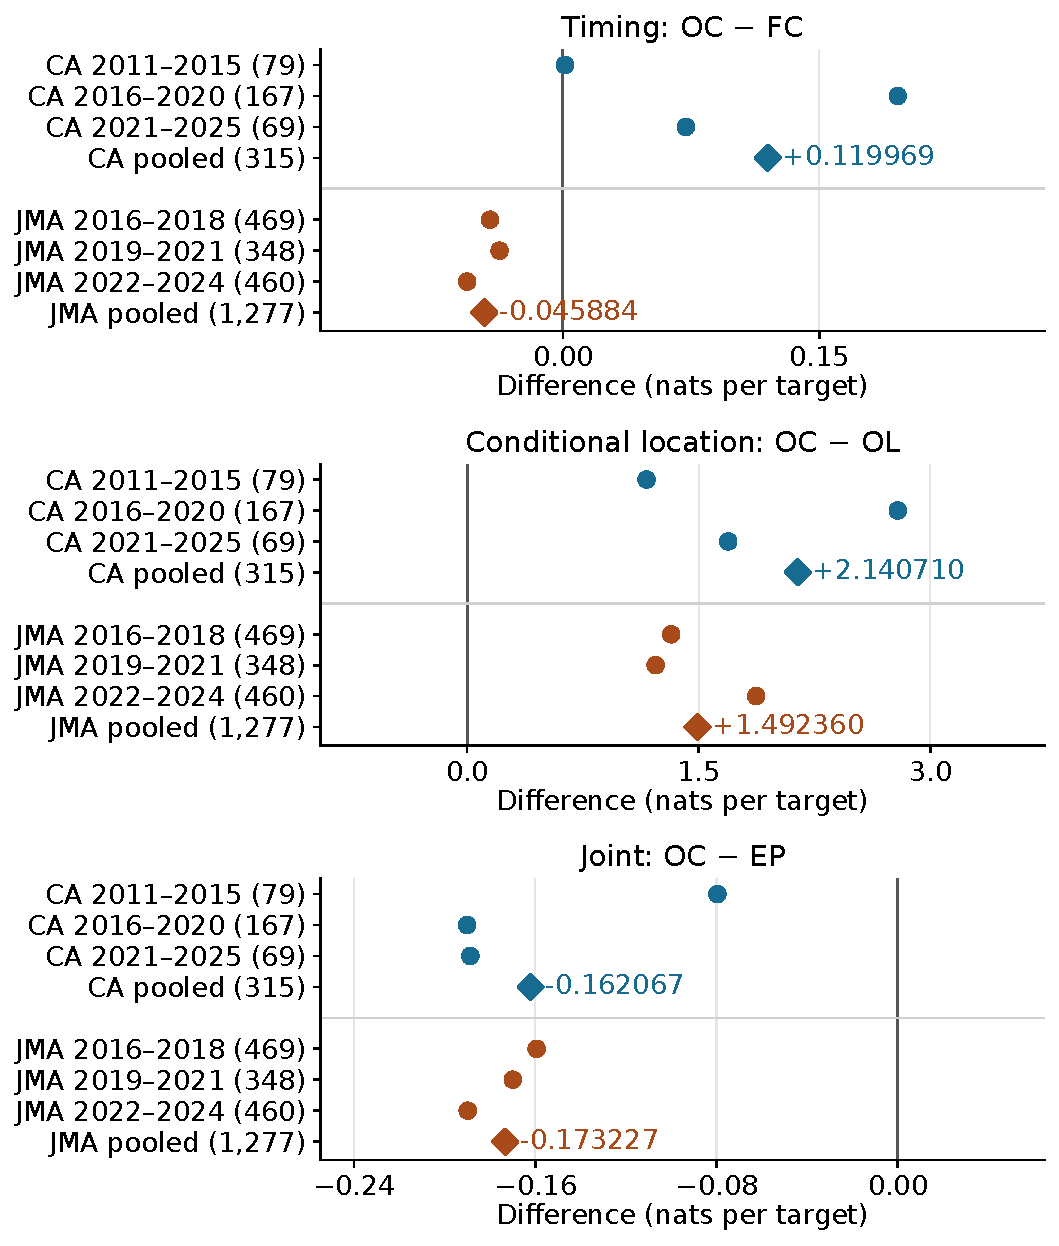
\includegraphics[width=\linewidth,height=.78\textheight,keepaspectratio]{spatial_addendum_iv_matched_regional_contrasts.pdf}
\caption{Matched timing and location comparisons in California and Japan. Realised proper-score contrasts from the original California M $\geq$ 4 cohort (315 targets) and the JMA reported-primary M $\geq$ 4.5 complete-case cohort (1,277 records). Each panel has its own reference and horizontal scale. Timing compares OC with FC; conditional location compares OC with OL; joint compares OC with EP. Pooled diamonds divide summed window nats by the regional total. California uses UTC years and JMA source-JST years. Different-reference columns and geographies are not added. Related retrospective windows have no event-iid uncertainty intervals.}\end{figure}



The California accepted report supplies source selection, repair chronology and complete comparison components.

\section{Stronger benchmarks change the conclusion}

OC exceeds the refitted N0 procedure by +1694.942967 joint nats over 315 targets, but EP exceeds OC in each primary California test window. The same 315 targets, common mark law and frozen OC states are used. EP was independently fitted using training data; it was not selected as a replacement downstream forecast after inspecting these scores.

\begingroup\footnotesize\setlength{\tabcolsep}{2pt}\renewcommand{\arraystretch}{1.18}
\begin{longtable}{@{}>{\raggedright\arraybackslash}p{0.1800\textwidth}>{\raggedright\arraybackslash}p{0.1800\textwidth}>{\raggedright\arraybackslash}p{0.1800\textwidth}>{\raggedright\arraybackslash}p{0.1800\textwidth}>{\raggedright\arraybackslash}p{0.1800\textwidth}@{}}
\toprule
{}OC minus reference, pooled 315 & Joint nats & Timing nats & Location nats & Joint nats/target \\
\midrule\endfirsthead
\toprule
OC minus reference, pooled 315 & Joint nats & Timing nats & Location nats & Joint nats/target \\
\midrule\endhead
\midrule\multicolumn{5}{r}{\emph{Continued on next page}}\\
\endfoot
\bottomrule\endlastfoot
{}N0 & +1694.94 & +894.846 & +800.097 & +5.38077 \\
{}EP & -51.0512 & +0.33625 & -51.3875 & -0.162067 \\
\end{longtable}\endgroup

OC-N0 joint, timing and location differences are positive in all three windows. This supplies a serious no-trigger predictive comparison that a numerical Poisson floor could not supply. Its middle window contributes about 77.49\% of the joint gain. The comparison is between complete procedures with shared trained geography; it does not establish causal triggering or identify immigrant labels.

OC-EP joint differences are -6.288819, -31.742512 and -13.019873 nats. Conditional location loses in each window. The pooled timing difference is only +0.001067 nats per target, with a small middle-window loss; EP's joint advantage is mainly spatial. Therefore the finding that OC improves on OL cannot be promoted into superiority over the strongest evaluated spatial benchmark.

The decomposition also matters. Against EP, the point-event difference is -54.591677 nats, partly offset by a +3.540472 signed exposure contribution. Against N0, these are +1612.690857 and +82.252111. A point-only comparison would omit quiet-period exposure. The common magnitude law contributes equally to every arm, so these joint-score contrasts measure space--time occurrence forecasting; all mark differences are zero.

\begin{figure}[tbp]\centering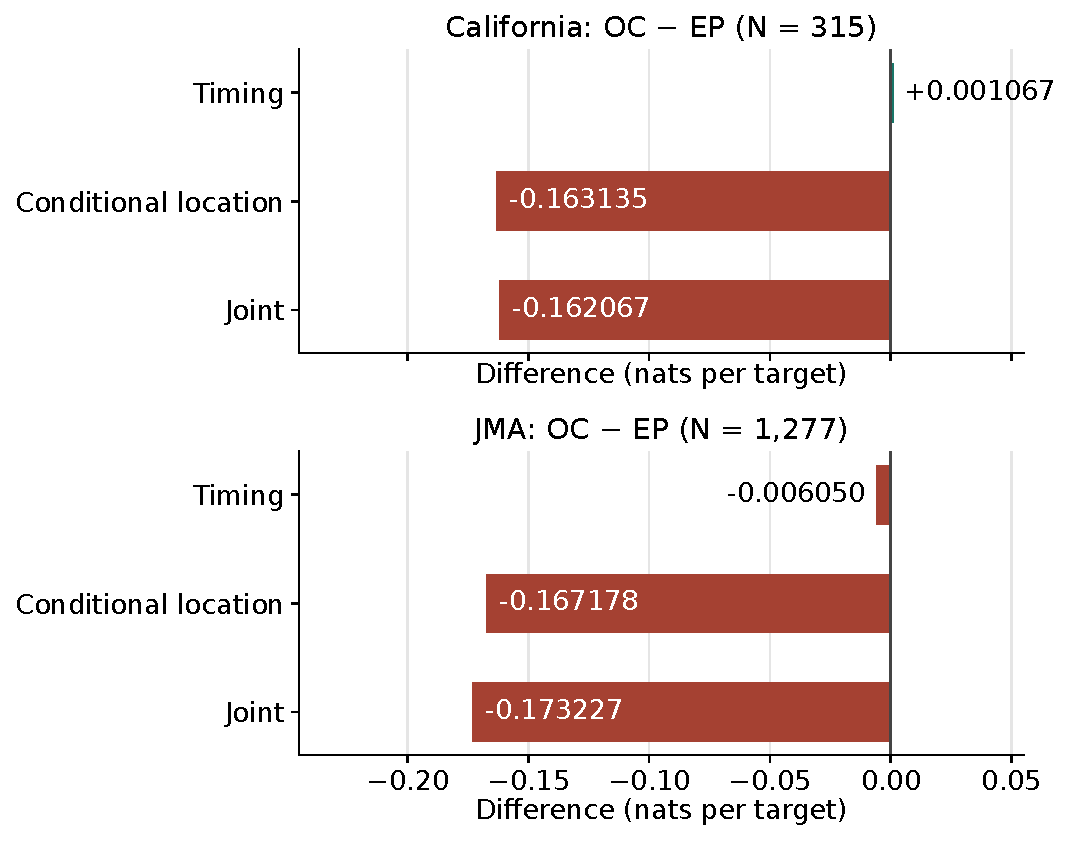
\includegraphics[width=\linewidth,height=.78\textheight,keepaspectratio]{spatial_addendum_iv_ep_score_components.pdf}
\caption{Timing and location components of OC relative to EP in California and Japan. Pooled OC-minus-EP timing, conditional-location and joint differences, normalized separately by 315 California targets and 1,277 JMA records. Joint equals timing plus conditional location because mark differences are zero. California has a tiny timing edge; JMA has a timing loss. The larger location deficit accounts for most joint loss in both regions. EP is a separately fitted complete procedure; relative superiority establishes neither EP calibration nor an isolated temporal-kernel effect.}\end{figure}



The competitive benchmark report is the numeric authority for this section. The LI replay in Chapter~\ref{ch:local-inhibition} is separately sourced and differs at floating-point scale; it does not replace these archived benchmark values.

\section{Conditional adequacy is a separate question}
The frozen OC conditional simulation and its complete coordinate results are developed in Chapter~\ref{ch:calibration}. Relative scores here do not supply an adequacy result for either OC or EP.
\section{Robustness and concentration answer narrower questions}

\subsection{A higher threshold retains directions under a changed observation law}

The base annual accounting retains every event's original history and all exposure, including years with zero targets. It refits no base parameter. A separately admitted M $\geq$ 4.5 sensitivity rebuilds the population, eligible histories, training estimates, mark law and fitted procedures. Its 391-record population includes 33 warmup parents; training counts are 271, 287 and 340, and test counts 16, 53 and 18, totaling 87. Those 87 are a higher-threshold subset of the California history, not 87 additional independent records to add to 315.

The sensitivity applies the threshold to the provider's exact preferred-magnitude token before converting magnitude excess to binary64. Its relative mark-bin cutoff remains 0.5, corresponding to M5.0. Domain, depth/type/time rules, strict earlier-parent eligibility and $r=0.7$ are retained. Beta, hierarchical reference masses, KDE bandwidth and model parameters are re-estimated from each training prefix. Six fixed-ML continuous spatial selectors, a lifted prerequisite, common-scale ML and the two Omori procedures remain in the roster; the selected fixed-ML arm is an alias of its winning selector, not an extra fit. The first fold served as the resource/correctness pilot, and its accepted files were reused without score-based continuation or replacement. The 87 targets fall below the inherited descriptive reference of 100 in total; 16 and 18 also fall below 20 per window. Those pragmatic references are not power guarantees.

\begingroup\footnotesize\setlength{\tabcolsep}{2pt}\renewcommand{\arraystretch}{1.18}
\begin{longtable}{@{}>{\raggedright\arraybackslash}p{0.1800\textwidth}>{\raggedright\arraybackslash}p{0.1800\textwidth}>{\raggedright\arraybackslash}p{0.1800\textwidth}>{\raggedright\arraybackslash}p{0.1800\textwidth}>{\raggedright\arraybackslash}p{0.1800\textwidth}@{}}
\toprule
{}Primary comparison and component & M $\geq$ 4.0 nats/target (315) & M $\geq$ 4.5 nats/target (87) & M $\geq$ 4.5 total nats & Positive windows \\
\midrule\endfirsthead
\toprule
Primary comparison and component & M $\geq$ 4.0 nats/target (315) & M $\geq$ 4.5 nats/target (87) & M $\geq$ 4.5 total nats & Positive windows \\
\midrule\endhead
\midrule\multicolumn{5}{r}{\emph{Continued on next page}}\\
\endfoot
\bottomrule\endlastfoot
{}OC-FC timing & +0.119969 & +0.152292 & +13.2494 & 3/3 \\
{}OC-OL location & +2.14071 & +2.12387 & +184.776 & 3/3 \\
{}OC-MC joint context & +0.0672314 & +0.0775184 & +6.7441 & 2/3 \\
\end{longtable}\endgroup

The first higher-threshold OC-MC joint difference is -0.626348 nats, and its OC-FC timing gain is only +0.077968 total nats. The two smaller test windows contain fewer than 20 targets. The threshold columns describe distinct complete procedures and target/parent laws; their difference is not a paired performance improvement or a threshold selection result. EP was not refitted or evaluated in this sensitivity, and no new calibration was performed.

Against OL, the higher-threshold location decomposition is +5.881781 zone, +2.472120 conditional-cell and +176.422568 within-cell nats. Its OC--FC timing decomposition is +14.762895 event-ground nats minus 1.513472 integrated-exposure nats; OC--MC joint gain comprises +5.992897 timing and +0.751200 location nats. Each decomposition retains its own reference.

Preferred magnitudes mix magnitude types and are not homogeneous moment magnitude. Count eligibility does not establish physical detection completeness. The source provides no defensible numerical location covariance or empirical location-error distribution; no perturbation law was invented from quality codes or decimal places. No independent alternate historical snapshot was admitted. The sensitivity therefore supports direction under one specified observation-law change, not general robustness to catalogue uncertainty.

\begin{figure}[tbp]\centering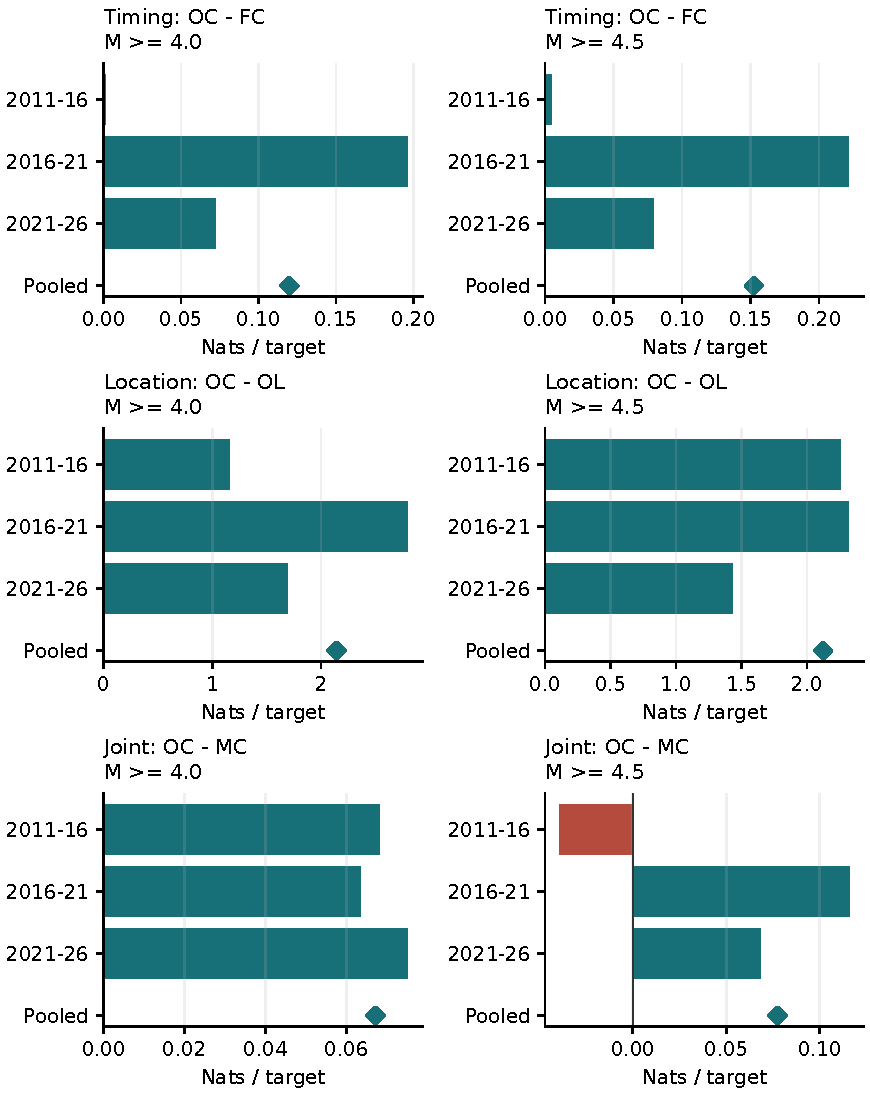
\includegraphics[width=\linewidth,height=.78\textheight,keepaspectratio]{spatial_detail_window_primary_nats_per_target_m4_m45_v1.pdf}
\caption{Fixed-window and event-weighted pooled primary score contrasts per target under M $\geq$ 4.0 and M $\geq$ 4.5. Bars retain the three windows and pooled diamonds divide summed nats by 315 or 87 targets. Each component uses its named reference; the negative early OC--MC joint contrast is retained. Cross-threshold differences are descriptive, not paired performance gains.}\end{figure}


\subsection{Annual gains are concentrated}

In the base analysis, calendar 2019 has 116 targets and contributes +29.280597 OC-FC timing nats, +392.773429 OC-OL location nats and +7.979400 OC-MC joint nats. At M $\geq$ 4.5, 37 targets in that year contribute +10.977080, +112.007721 and +5.288450 respectively. These are separate contrast/component columns. Negative annual contributions remain in the accepted tables.

The base 2019 signed shares are 77.48\%, 58.247\% and 37.678\% of their respective pooled contrasts, including negative years in each denominator. At the higher threshold, ten of fifteen annual timing contributions are negative. Zero-target years 2015 and 2017 retain their exposure terms; their per-target means are undefined, not zero. Appendix~\ref{app:audit11-annual} retains every annual row and both thresholds.

Annual partitions preserve subsequent parent history. They do not estimate a counterfactual catalogue without a sequence. Their purpose is to locate realised score contributions, not to remove inconvenient years or create independent replications. The robustness decision report records the full design and absent sensitivity laws.

\begin{figure}[tbp]\centering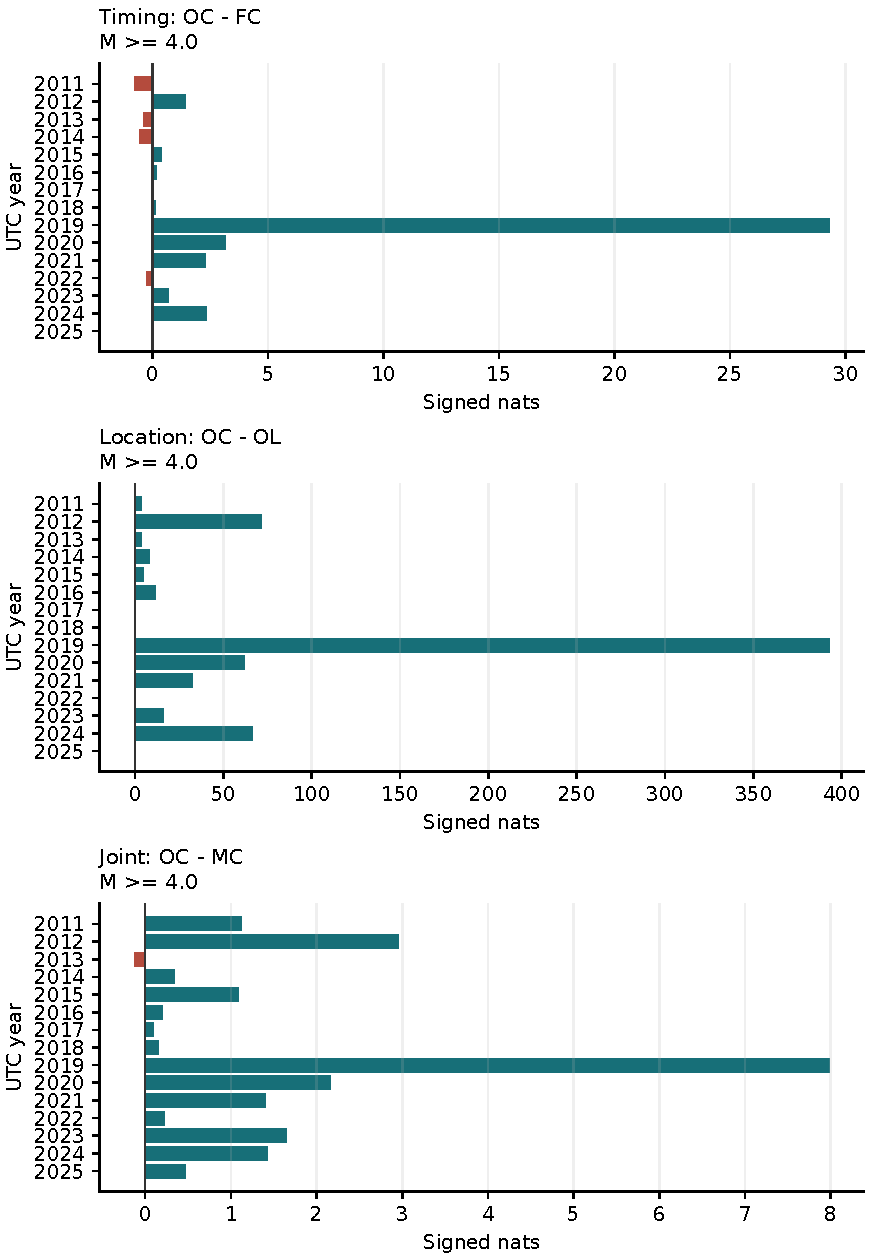
\includegraphics[width=\linewidth,height=.78\textheight,keepaspectratio]{spatial_detail_annual_primary_contributions_v1.pdf}
\caption{Annual signed score contributions for all fifteen California M $\geq$ 4.0 test years under the three distinct named comparisons. The panels use their own references; negative years remain. These are contributions to realised scores, not independent annual replications.}\end{figure}

\begin{figure}[tbp]\centering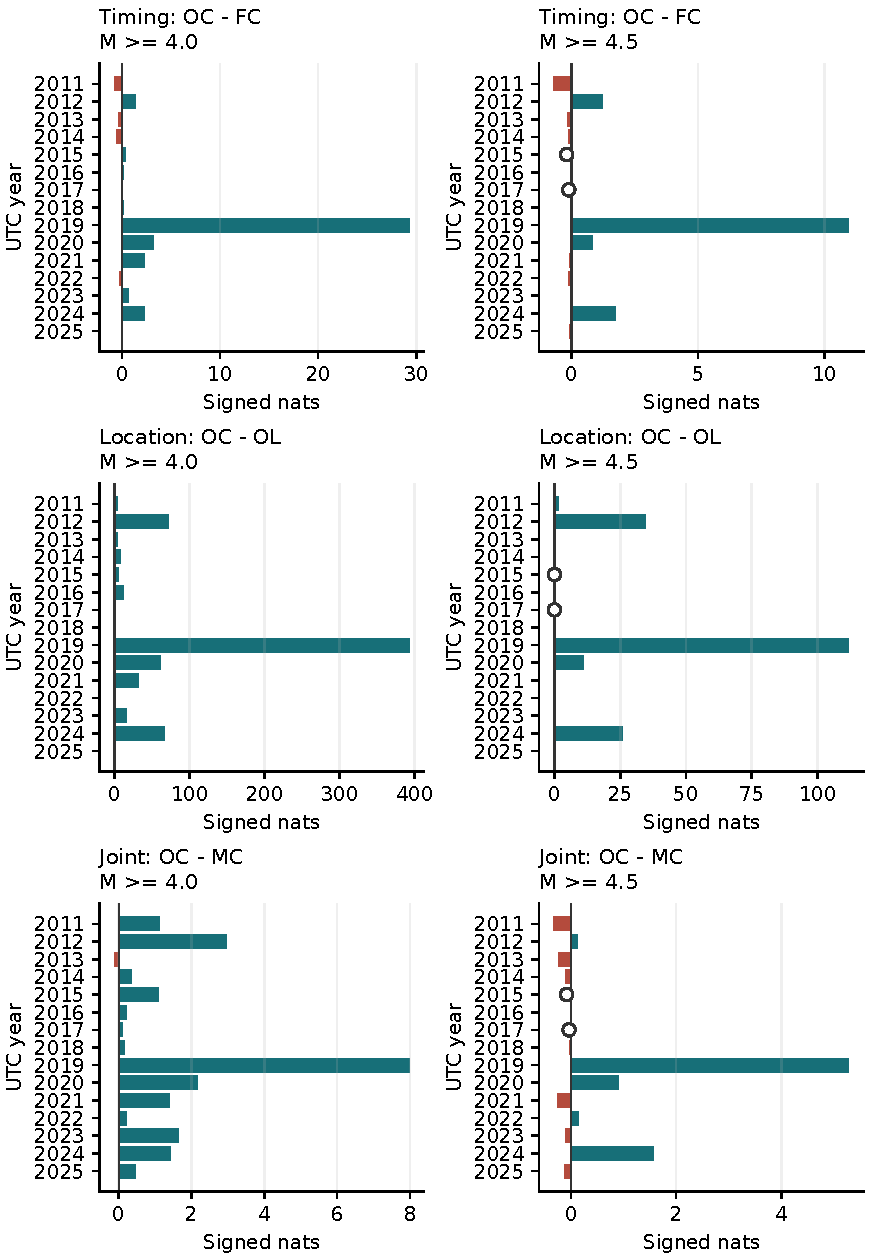
\includegraphics[width=\linewidth,height=.78\textheight,keepaspectratio]{spatial_detail_annual_primary_contributions_m4_m45_v1.pdf}
\caption{Annual signed score contributions under M $\geq$ 4.0 and M $\geq$ 4.5. All fifteen years remain; hollow circles identify zero-target years whose exposure contributions are retained. Component panels have distinct references. The nested populations and refitted procedures do not define a paired threshold gain.}\end{figure}


\subsection{One eligible active episode, with the complete complement retained}
\label{sec:calendar-sequence-partition}

The finer sequence partition was chosen after annual inspection, including 2019. The frozen metadata rule marks regional time active when an admissible M $\geq$ 6 anchor at u satisfies u < t $\leq$ u + 30 days. Overlapping anchor windows merge globally before fold clipping; eligible prehistory is retained. This is a regional time partition, not a causal or spatial aftershock classification. The initial anchor belongs to the complement unless an earlier anchor already activates it.

Only one eligible episode intersects the scored test windows: a Ridgecrest-associated union lasting 31.406991204 days with 110 targets. The other 205 targets and 5,447.593008796 exposure days remain the complete complement. Thirteen anchors and ten global episodes occur in the admitted chronology, but nine episodes lie in pre-test history. They are not nine additional scored replications.

The active period contributes +30.058155064 of the +37.790339259 pooled OC--FC timing nats, approximately 79.54\%. With only one scored episode, the archive cannot estimate reproducibility of that concentration across sequences. Integer UTC membership and global interval merging are fixed before fold clipping. One of the two test anchor targets is active and the other is in the complement; event-only anchor scores are not part of the public aggregate.

\begingroup\footnotesize\setlength{\tabcolsep}{2pt}\renewcommand{\arraystretch}{1.18}
\begin{longtable}{@{}>{\raggedright\arraybackslash}p{0.1800\textwidth}>{\raggedright\arraybackslash}p{0.1800\textwidth}>{\raggedright\arraybackslash}p{0.1800\textwidth}>{\raggedright\arraybackslash}p{0.1800\textwidth}>{\raggedright\arraybackslash}p{0.1800\textwidth}@{}}
\toprule
{}Pooled category & Targets & OC-FC timing nats & OC-OL location nats & OC-MC joint nats \\
\midrule\endfirsthead
\toprule
Pooled category & Targets & OC-FC timing nats & OC-OL location nats & OC-MC joint nats \\
\midrule\endhead
\midrule\multicolumn{5}{r}{\emph{Continued on next page}}\\
\endfoot
\bottomrule\endlastfoot
{}Active period & 110 & +30.0582 & +375.945 & +9.87815 \\
{}Complete complement & 205 & +7.73218 & +298.379 & +11.2997 \\
{}Full original pool & 315 & +37.7903 & +674.324 & +21.1779 \\
\end{longtable}\endgroup

The six-target calendar-2019 complement is the non-active portion of the 116-target UTC calendar year 2019 within primary Fold 1, distinct from the 127-target causal-origin block and its 16-target complement in Section~\ref{sec:s06-completed}. This calendar-year complement has -0.777558 timing nats and -1.898745 OC-MC joint nats, although its location contribution is positive. The annual timing and MC-context gains therefore arise in the active period. Across the full fifteen test years, all three contextual totals remain positive in the complement; concentration does not mean every contextual gain is confined to that episode.

The stronger reference still wins both partitions. OC-EP joint score is -18.372230 nats in the active period and -32.678975 in the complete complement. Its active timing difference is -0.806683 and location difference -17.565547. Complement timing is +1.142932, outweighed by -33.821907 location nats. All original parents and full-domain exposure remain in every score; event-only scoring would answer a different question. The sequence audit report retains empty active rows, exact exposure accounting and the full partition.

The complete partition tables in Appendix~\ref{app:audit11-sequence} retain empty active periods, full-domain exposures and absolute arm scores. Calendar-2019 and pooled rows repeat portions of the original folds for reporting and must not be added to them. The sequence partition changes neither the original fifteen selected states nor their eligible parent histories.

\section{Japan: spatial direction transfers, combined criterion does not}

\subsection{The reported-record target}

The JMA analysis processes 19 local annual archives for source-JST years 2006-2024. Its 4,019,138 source records yield 4,602 usable study records. The target requires agency J, natural subsidiary 1, determination K/k/A, allowed primary magnitude types J/D/V/d/v, observed numeric primary reported M $\geq$ 4.5, depth 0-60 km and the fixed projected region. Primary and secondary magnitudes remain separate. This is an observed primary complete-case reported-record cohort, not homogeneous Mw, inferred latent magnitudes or proof of physical completeness.

Inspection identified 41,278 initially unresolved target observations: 41,277 with missing/undetermined primary information alone and one with an additional depth issue. An explicit, inspection-informed restriction requires numeric observed primary magnitude and an allowed primary type. It was documented and independently reviewed before fitting. Those records receive no assigned latent magnitude and are not asserted to be physically small. No complete target row was added, removed or modified by that clarification. One auxiliary depth-ambiguous subthreshold record remains unusable for diagnostics and has zero target, parent or beta-observation effect.

The 496 records in 2006-2010 supply warmup only. The following training prefixes and disjoint test windows use exact source-JST boundaries.

\begingroup\footnotesize\setlength{\tabcolsep}{2pt}\renewcommand{\arraystretch}{1.18}
\begin{longtable}{@{}>{\raggedright\arraybackslash}p{0.1800\textwidth}>{\raggedright\arraybackslash}p{0.1800\textwidth}>{\raggedright\arraybackslash}p{0.1800\textwidth}>{\raggedright\arraybackslash}p{0.1800\textwidth}>{\raggedright\arraybackslash}p{0.1800\textwidth}@{}}
\toprule
{}Origin & Scored training years & Training records & Test years & Test records \\
\midrule\endfirsthead
\toprule
Origin & Scored training years & Training records & Test years & Test records \\
\midrule\endhead
\midrule\multicolumn{5}{r}{\emph{Continued on next page}}\\
\endfoot
\bottomrule\endlastfoot
{}2016 & 2011-2015 & 2,829 & 2016-2018 & 469 \\
{}2019 & 2011-2018 & 3,298 & 2019-2021 & 348 \\
{}2022 & 2011-2021 & 3,646 & 2022-2024 & 460 \\
\end{longtable}\endgroup

The total scored denominator is 1,277. These are revised local records; catalogue inspection and observation adjudication preclude a pristine as-issued holdout claim. The JMA processing report gives the source restrictions and exact accounting.

\subsection{Descriptive transfer rule and competitive context}

The combined descriptive transfer rule requires both primary contrasts to exceed +0.0006 pooled total nats and each to be positive in at least two of three folds after audit pass. That threshold allows the declared numerical score tolerance; it is not a statistical significance boundary. The EP joint comparison is separate competitive context.

The $0.0006$ threshold allows $0.0001$ nat for each of two arm scores across three folds. It is a numerical comparison rule, not evidence that the three windows or their events are independent tests.

\begingroup\footnotesize\setlength{\tabcolsep}{2pt}\renewcommand{\arraystretch}{1.18}
\begin{longtable}{@{}>{\raggedright\arraybackslash}p{0.1800\textwidth}>{\raggedright\arraybackslash}p{0.1800\textwidth}>{\raggedright\arraybackslash}p{0.1800\textwidth}>{\raggedright\arraybackslash}p{0.1800\textwidth}>{\raggedright\arraybackslash}p{0.1800\textwidth}@{}}
\toprule
{}Comparison and component & Total nats & Nats/record (1,277) & Direction in windows & Interpretation \\
\midrule\endfirsthead
\toprule
Comparison and component & Total nats & Nats/record (1,277) & Direction in windows & Interpretation \\
\midrule\endhead
\midrule\multicolumn{5}{r}{\emph{Continued on next page}}\\
\endfoot
\bottomrule\endlastfoot
{}OC-FC timing & -58.5935 & -0.0458837 & Negative 3/3 & Timing direction reverses \\
{}OC-OL location & +1905.74 & +1.49236 & Positive 3/3 & Spatial direction transfers \\
{}OC-EP joint & -221.211 & -0.173227 & Negative 3/3 & Strong reference still wins \\
{}OC-MC joint context & -49.1946 & -0.0385236 & Negative 3/3 & No universal Omori preference \\
{}FC-FL location context & +1847.64 & +1.44686 & Positive 3/3 & Spatial result also under FC \\
\end{longtable}\endgroup

The registered combined criterion is \textbf{not demonstrated}. OC-FC timing losses are approximately -19.9765, -12.8718 and -25.7452 nats. OC-OL location gains are approximately +619.711, +424.797 and +861.235. A large location total cannot compensate for a timing requirement with the wrong sign, and primary contrasts with different references must not be added.

EP exceeds OC jointly in all three windows. Conditional location accounts for 213.485907 of the 221.211492-nat deficit. OC also exceeds N0 on pooled joint score, but the strong-reference failure remains. These findings support a useful continuous-versus-lifted representation contrast while qualifying temporal transfer and overall competitive performance.

All background bandwidth selectors choose the lower 5 km endpoint, while FC spatial-scale selectors choose the interior 15 km value. The background trend slope reaches its lower bound for 7, 6 and 2 of seven models in the three folds. Results apply to the frozen grids and bounds; these choices do not identify physical length scales or measurement precision. The JMA forecast report retains full components, annual accounting and the registered decision.

Appendix~\ref{app:audit11-jma} retains all seven pooled contrasts and their three window differences, including OC--FL and OC--N0. The nine annual source-JST blocks retain the same counts and all canonical score/exposure components. No Powell recovery was needed for the 288 accepted L-BFGS-B returns. The filesystem retry reused seven completed procedures byte-for-byte and restored one written floor without reevaluation; it did not change the scientific objective or selection rule.

\section{Consolidated implications and limits}

The completed evidence separates five conclusions. First, continuous offspring geography repeatedly improves conditional location relative to the declared cell-lift procedure, including California's higher-threshold sensitivity and the JMA reported-record cohort. Second, Omori's timing advantage over fixed-scale ML is conditional: positive in the original New Zealand/California comparisons, but negative in every JMA window. Third, excitation improves relative scores over a serious refitted no-trigger baseline, while EP beats OC on joint score in the primary California and Japan folds, mainly through location. Fourth, OC's conditional diagnostics disclose material discrepancies, so relative gains are not adequate-probability certification. Fifth, California gains are uneven and concentrated, with only one eligible scored sequence period and substantial full-complement contributions.

The historical archives have been inspected, processed and revised; later studies adaptively reuse outcomes and related chronological windows. Frozen training/test calculations within a study do not erase that programme-level reuse. Overlapping training prefixes, earthquake dependence and small numbers of windows preclude event-iid confidence intervals and broad independent-replication claims. No Wilks inference, causal triggering claim, recovered immigrant law, physical stress range or absolute calibration result follows. Magnitude-type mixtures, reported-coordinate observation laws, finite-domain parent omissions, plug-in background estimates and grid/boundary choices remain material.


\section{Numerical custody and review scope}

Numerical agreement supports the reported calculations; it does not independently replicate earthquake science. The California source repair accounted for 30 procedures and 240 starts. The separate benchmark audited all six new fit procedures and reconciled scores within 8.19e-11 nats. The higher-threshold sensitivity accounted for 30 procedures and 240 starts, reconciling within 1.13e-11 nats. The sequence audit retained all 315 targets and passed 7,128 component checks with maximum discrepancy 4.55e-13 nats. These are different validation rosters and are not independent research samples to add together.

JMA fitting resolved 36 procedures, 288 starts, 42 floors and 330 slots. Maximum independently reconstructed score disagreement was 1.82e-10 nats against a 1e-4-nat tolerance; maximum stored near-optimal spread was 3.75e-5 nats per record against a strict 0.01 gate. A retained atomic-save interruption was repaired by bounded filesystem retry, preserving completed states without refitting. Other historical failures and recoveries remain in the source reports. Multistart completion and near-optimal-set stability are not global optimization certificates or uncertainty intervals.

The public reproduction bundle now reconstructs the California and Japan cohorts from the original provider records, including source-row identities, exclusion accounting, exact clocks and chronological partitions. The Japanese bundle also supplies recovered fitted states and the explicit projected-region predicate. The current evidence index retains the source pins, unchanged display scalars, source-specific field dictionary and claim bindings. The readable scientific protocol subset supplies the LI law, clocks and fitting contract used in Chapter~\ref{ch:local-inhibition}. The review guide separates these executed cohort replays from regional model refitting and scoring; rebuilding a cohort does not itself rerun its benchmark fits. Rebuildable event caches are outputs of the numerical pipeline, rather than required private inputs.

The detailed numerical record is organized once in Appendix~\ref{app:audit11}. It contains the annual, higher-threshold, sequence-partition and JMA backup tables, with their source-specific denominators and exposure signs; the standalone decision-report narratives are not repeated here.


\section{Completed four-arm spatial comparison}

\label{sec:s03-completed}

\textit{Numerical status: all folds passed their saved custody and score-decomposition checks, and the predeclared independent California-fold sample passed. Acceptance uses sampled validation, not independent raw replay of every fit.}

The comparison contains three California folds with 315 targets and three New Zealand folds with 612 targets. Four procedures are evaluated in each fold: arm 1 uses the reference-density-weighted rational offspring kernel and inherited KDE background; arm 2 removes reference-density weighting; arm 3 adds identity-based leave-one-out background fitting; arm 4 uses the unweighted EP offspring shape with the inherited background procedure. The temporal and mark parameters remain training-selected and fixed. Background level, trend and reproduction coefficient are refitted under the declared arm-specific normalization. California uses the archived training-selected EP spatial scale and shape. The New Zealand OC archives did not contain EP spatial parameters, so a separate training-only prerequisite estimated these missing nuisance parameters before the four-arm comparison. Those values were then frozen: each final arm optimizes only background level, trend and reproduction coefficient. This prerequisite is an explicit addition to the original execution specification, not a claim that the entire preparation fitted only three parameters.

\begin{table}[htbp]\centering

\caption{Held-out joint log-score contrasts in nats. Positive values favour the first named arm. Arm labels follow the text.}\label{tab:s03-completed}

\begin{tabular}{llrrrrr}\toprule Region & Fold & Targets & $2-1$ & $3-2$ & $4-2$ & $4-1$\\\midrule

CA & 0 & 79 & -0.2962 & 1.4515 & 6.3629 & 6.0668 \\

CA & 1 & 167 & 1.0722 & 3.1070 & 29.9884 & 31.0606 \\

CA & 2 & 69 & 0.2776 & 0.7288 & 12.6035 & 12.8811 \\

NZ & 0 & 203 & 0.3421 & 2.1881 & 17.9074 & 18.2495 \\

NZ & 1 & 155 & 33.2980 & -0.3822 & -0.0583 & 33.2397 \\

NZ & 2 & 254 & -1.2518 & -3.2235 & 0.0346 & -1.2172 \\

\bottomrule\end{tabular}\end{table}

\begin{table}[htbp]\centering

\caption{Regional totals for EP minus the OC baseline, in nats. The common mark score cancels.}

\begin{tabular}{lrrr}\toprule Region & Timing & Location & Joint\\\midrule

CA & -0.8205 & 50.8289 & 50.0085 \\

NZ & 2.1452 & 48.1269 & 50.2721 \\

\bottomrule\end{tabular}\end{table}

The contrasts are descriptive comparisons of fitted procedures, not additive causal contributions. In particular, arm 4 minus arm 3 changes the offspring model and the background fitting procedure; it is not a pure tail effect. Arm 4 minus arm 2 is the direct EP versus unweighted-rational comparison with the same background procedure. The identity $(4-1)=(2-1)+(3-2)+(4-3)$ is exact bookkeeping, whereas $(2-1)+(3-2)+(4-2)$ is not the total. Refitting the shared nuisance coefficients further prevents a mechanical causal attribution to a single feature.

All finite retained-state and near-optimal forecast checks are supplied in \path{reproduction/regional/original_completion_20261101.zip}, with planned denominators retained. The closure verification checks the exact frozen spatial parameters, common temporal and mark parameters, three-coordinate final fits, and training-only winner selection across all six folds. It verifies original and portable case byte identities separately and requires exact parsed-content equality; serialization differences are not treated as changed scientific inputs. This is retrospective verification of the saved contract, not a new fit or a fresh validation cohort. The acceptance plan combines a predeclared independent raw geometry/score sample for California fold zero with saved custody, start coverage, selection and score-decomposition checks across all folds. It does not claim independent raw replay of every fit or New Zealand shape prerequisite. New Zealand results retain the archive-reuse disclosure; they are not a fresh untouched holdout.

\begin{figure}[htbp]\centering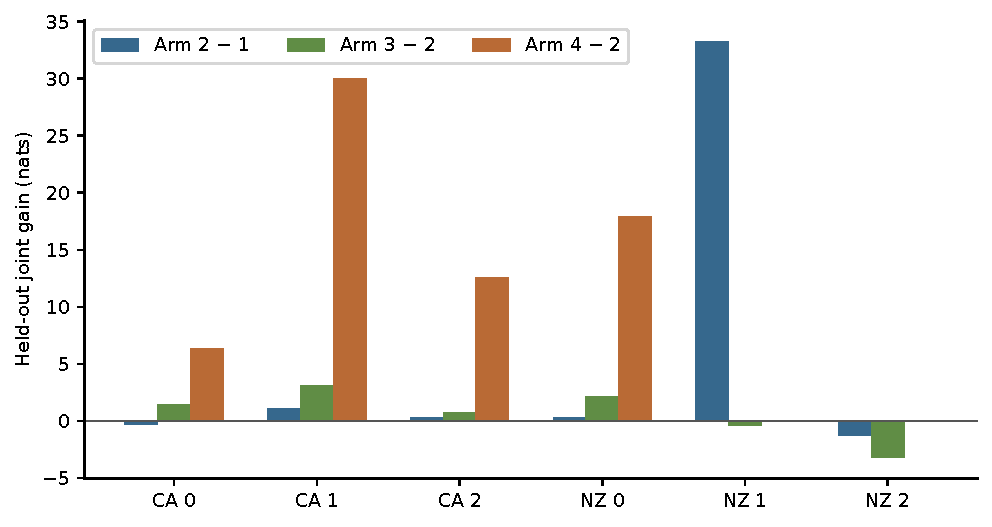
\includegraphics[width=\textwidth]{s03_completed_joint_contrasts.pdf}\caption{Saved held-out joint contrasts across all six folds. Each fold has its own refitted nuisance coefficients; these differences are not a causal mechanism decomposition. Saved custody checks and independent sampled raw validation passed.}\end{figure}


\section{Causal-window California backtests and JMA trend ablation}

\label{sec:s06-completed}

The California and JMA values in this section are recovered original fit and score outputs with checked hashes and source identities. The fitting and rescoring described below belong to the original study; this edition does not recompute them. The original audit coverage is retained.

The completed California map contains five eligible episodes, in 1994, 1999, 2004, 2010 and 2019. The two 1992 episodes are excluded by the predeclared training-count or zone-adequacy rule, not silently replaced by a more favourable sequence. Training expands from 1986 up to, but not including, each episode origin; the parent history retains the 1981 warmup. Each scored block ends at the earlier of the next eligible origin, one year after its origin, or the coverage cutoff. Parameters, spatial scale and nuisance inputs are selected only on the preceding training prefix.

The $M\geq6$ episode origins were identified retrospectively from the catalogue. The roster is retrospective and exploratory. Overlapping training histories and a common archive mean that the five episodes are not independent replications. The active partition is the union of declared episode time intervals, and its complement fills the rest of the scored block; it does not causally label individual earthquakes as aftershocks.

\begin{table}[htbp]\centering\caption{Held-out joint scores (nats) on the five eligible California blocks. Higher is better. These descriptive scores have no confidence intervals.}\label{tab:s06-ca}

\begin{tabular}{lrrrrr}\toprule Year & Targets & FC & MC & OC & EP\\\midrule

1994 & 64 & -527.0462 & -525.5013 & -526.7452 & -521.5603 \\

1999 & 75 & -551.4448 & -545.6841 & -540.1365 & -521.8412 \\

2004 & 30 & -349.2570 & -347.5086 & -347.8333 & -341.1560 \\

2010 & 125 & -1044.6385 & -1055.3761 & -1050.2614 & -1059.1042 \\

2019 & 127 & -696.3825 & -679.3514 & -670.2133 & -647.9267 \\

\bottomrule\end{tabular}\end{table}

\begin{table}[htbp]\centering\caption{OC minus FC joint contrasts, partitioned without changing fitted parameters. Full equals active plus complement, subject to the saved numerical tolerance. These contrasts are descriptive; no confidence intervals are supplied.}

\begin{tabular}{lrrrrr}\toprule Year & Active $N$ & Complement $N$ & Full & Active & Complement\\\midrule

1994 & 49 & 15 & 0.3010 & -0.0672 & 0.3682 \\

1999 & 61 & 14 & 11.3083 & 11.3970 & -0.0887 \\

2004 & 7 & 23 & 1.4237 & -0.1897 & 1.6134 \\

2010 & 75 & 50 & -5.6229 & -6.0147 & 0.3918 \\

2019 & 111 & 16 & 26.1693 & 26.3067 & -0.1374 \\

\bottomrule\end{tabular}\end{table}

EP achieves the highest held-out joint score in the 1994, 1999, 2004 and 2019 blocks, but loses in the 2010 block. That block contains 125 targets: 75 active and 50 in the complement.

EP's joint score of -1059.1042 is below OC (-1050.2614), FC (-1044.6385) and MC (-1055.3761). OC also trails FC: its joint contrast is -5.6229 nats, comprising -6.0147 active nats and 0.3918 complement nats. EP's joint advantage in the three primary chronological folds is therefore not uniform across every retrospective episode block.

The 2019 episode block contains 127 targets (111 active and 16 in the complement). It starts at the $M\geq6$ episode origin and runs for one year, so its denominator differs from the UTC calendar-2019 slice in Section~\ref{sec:calendar-sequence-partition}.

For JMA, the free-trend states are the preserved training-selected parameters, rescored without gratuitous refitting. The stationary alternative fixes $d=0$ and refits the prescribed starts and floors under the same training nuisance inputs. Both trends use identical target populations, the reported magnitude-lattice counting measure and all 1,277 targets across the three folds.

\begin{table}[htbp]\centering\caption{JMA contrasts (nats) under free and stationary background trend. Positive values favour OC. These contrasts are descriptive; no confidence intervals are supplied.}\label{tab:s06-jma}

\begin{tabular}{llrrrr}\toprule Fold & Trend & Targets & OC--FC timing & OC--EP timing & OC--EP joint\\\midrule

0 & free & 469 & -19.9765 & -1.1943 & -74.7591 \\

0 & $d=0$ & 469 & -20.0603 & -5.8012 & -76.4264 \\

1 & free & 348 & -12.8718 & -1.4445 & -59.1334 \\

1 & $d=0$ & 348 & -8.1665 & -4.1719 & -61.1146 \\

2 & free & 460 & -25.7452 & -5.0868 & -87.3190 \\

2 & $d=0$ & 460 & -9.6847 & -3.6114 & -84.6859 \\

\midrule

All & free & 1277 & -58.5935 & -7.7256 & -221.2115 \\

All & $d=0$ & 1277 & -37.9115 & -13.5846 & -222.2269 \\

\bottomrule\end{tabular}\end{table}

These ablation contrasts diagnose sensitivity to the fitted trend within the declared procedures. They do not isolate a physical mechanism, certify global optimization, or establish independent cross-region validation. Saved acceptance checks cover source and cache identities, causal windows, retained parent prefixes, required start/floor coverage, selected parameter reuse, numerical refinement, proper-score identities and the complete temporal partition. No independent likelihood replay is claimed by this completion check.

Fixing the background trend at zero reduces the pooled OC--FC timing deficit but does not eliminate it. The OC--EP joint deficit also persists, so a lower-bound trend estimate alone does not explain the Japanese reversal.

New Zealand remains an adaptively reused archive in this manuscript. S06 supplies no fresh New Zealand cohort and does not remove the adaptive-reuse disclosure or the need for genuinely prospective validation.

\begin{figure}[htbp]\centering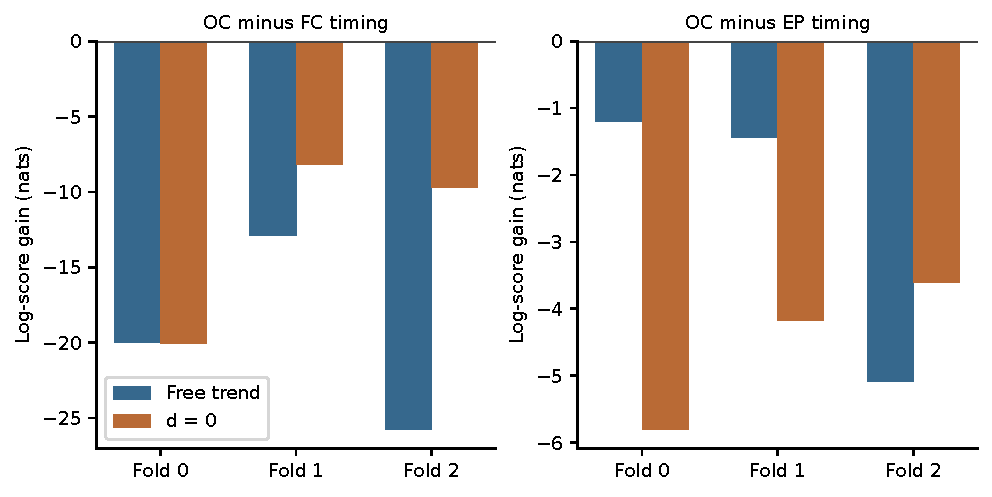
\includegraphics[width=\textwidth]{s06_jma_trend_timing.pdf}\caption{Saved JMA timing contrasts under free and stationary background trends. Each bar uses the same fold population; no new likelihood calculation or simulation was performed for the plot.}\end{figure}

